\documentclass{article}

\usepackage[utf8]{inputenc}
\usepackage{amsfonts}
\usepackage{amsmath}
\usepackage{graphicx}
\usepackage{amsthm}
\usepackage{soul}
\usepackage{hyperref}


\title{Final Results} 
\author{Samantha Mayers, srm2204@columbia.edu}% YOUR UNI GOES HERE
\date{October 24, 2020} % DATE GOES HERE
\maketitle

\begin{document}

\newpage
\section*{Objective}
The objective of this project was to determine how to accurately approximate Gaussian curves, with the goal of speeding up calculating an atomic PDF. \\

\section*{Terminology}
OG : Original Gaussian (the Gaussian which will be approximated) \\
Mini Gaussians: The smaller Gaussians that when summed, form an approximation for the original Gaussian \\ 
Approximation: The approximation formed from summing the mini Gaussians \\
Smaller Standard Deviation: The standard deviation used for all the mini Gaussians \\
Ratio: The ratio of the smaller standard deviation to the OG's standard deviation \\

\section*{Method}
The method used was multiple linear regression. Each curve, using a given "small" standard deviation, had generated the intensities of a number of smaller Gaussians (all with the same "smaller" standard deviation), such that when summed together, would yield an approximation of the original Gaussian. \\
\newline
Two different approaches were taken. First, the number of mini Gaussians generated per curve was held constant, at 5. However, as the ratio of the smaller standard deviation to the OG's standard deviation decreased, the accuracy of the approximation plummeted. One way to correct for this drawback is to continually reset the smaller standard deviation as the OG's standard deviation increases. If the data's standard deviations are within a reasonably small ratio, no resets or few resets would be necessary, making this first approach useful for that situation. \\
\newline
The second approach taken was to vary the number of Gaussians generated per curve. For standard deviation ratios (smallest standard deviation/OG's standard deviation) greater than .6 (number taken from Coelho paper), 5 mini Gaussians were used. If the standard deviation ratio was less than .6, 10 Gaussians were used. For this approach, no resets of the smaller standard deviation are necessary. \\

\newpage
\section*{Results}
Here are some figures demonstrating the results of the approximation technique. \\
\subsection*{Method 1: Constant Number of Mini Gaussians} 
First, the constant number of mini Gaussians approach: \\
\subsubsection*{No Resets} 
Within Method 1, first a look at the constant number of mini Gaussians approach with no smaller standard deviation resets: \\
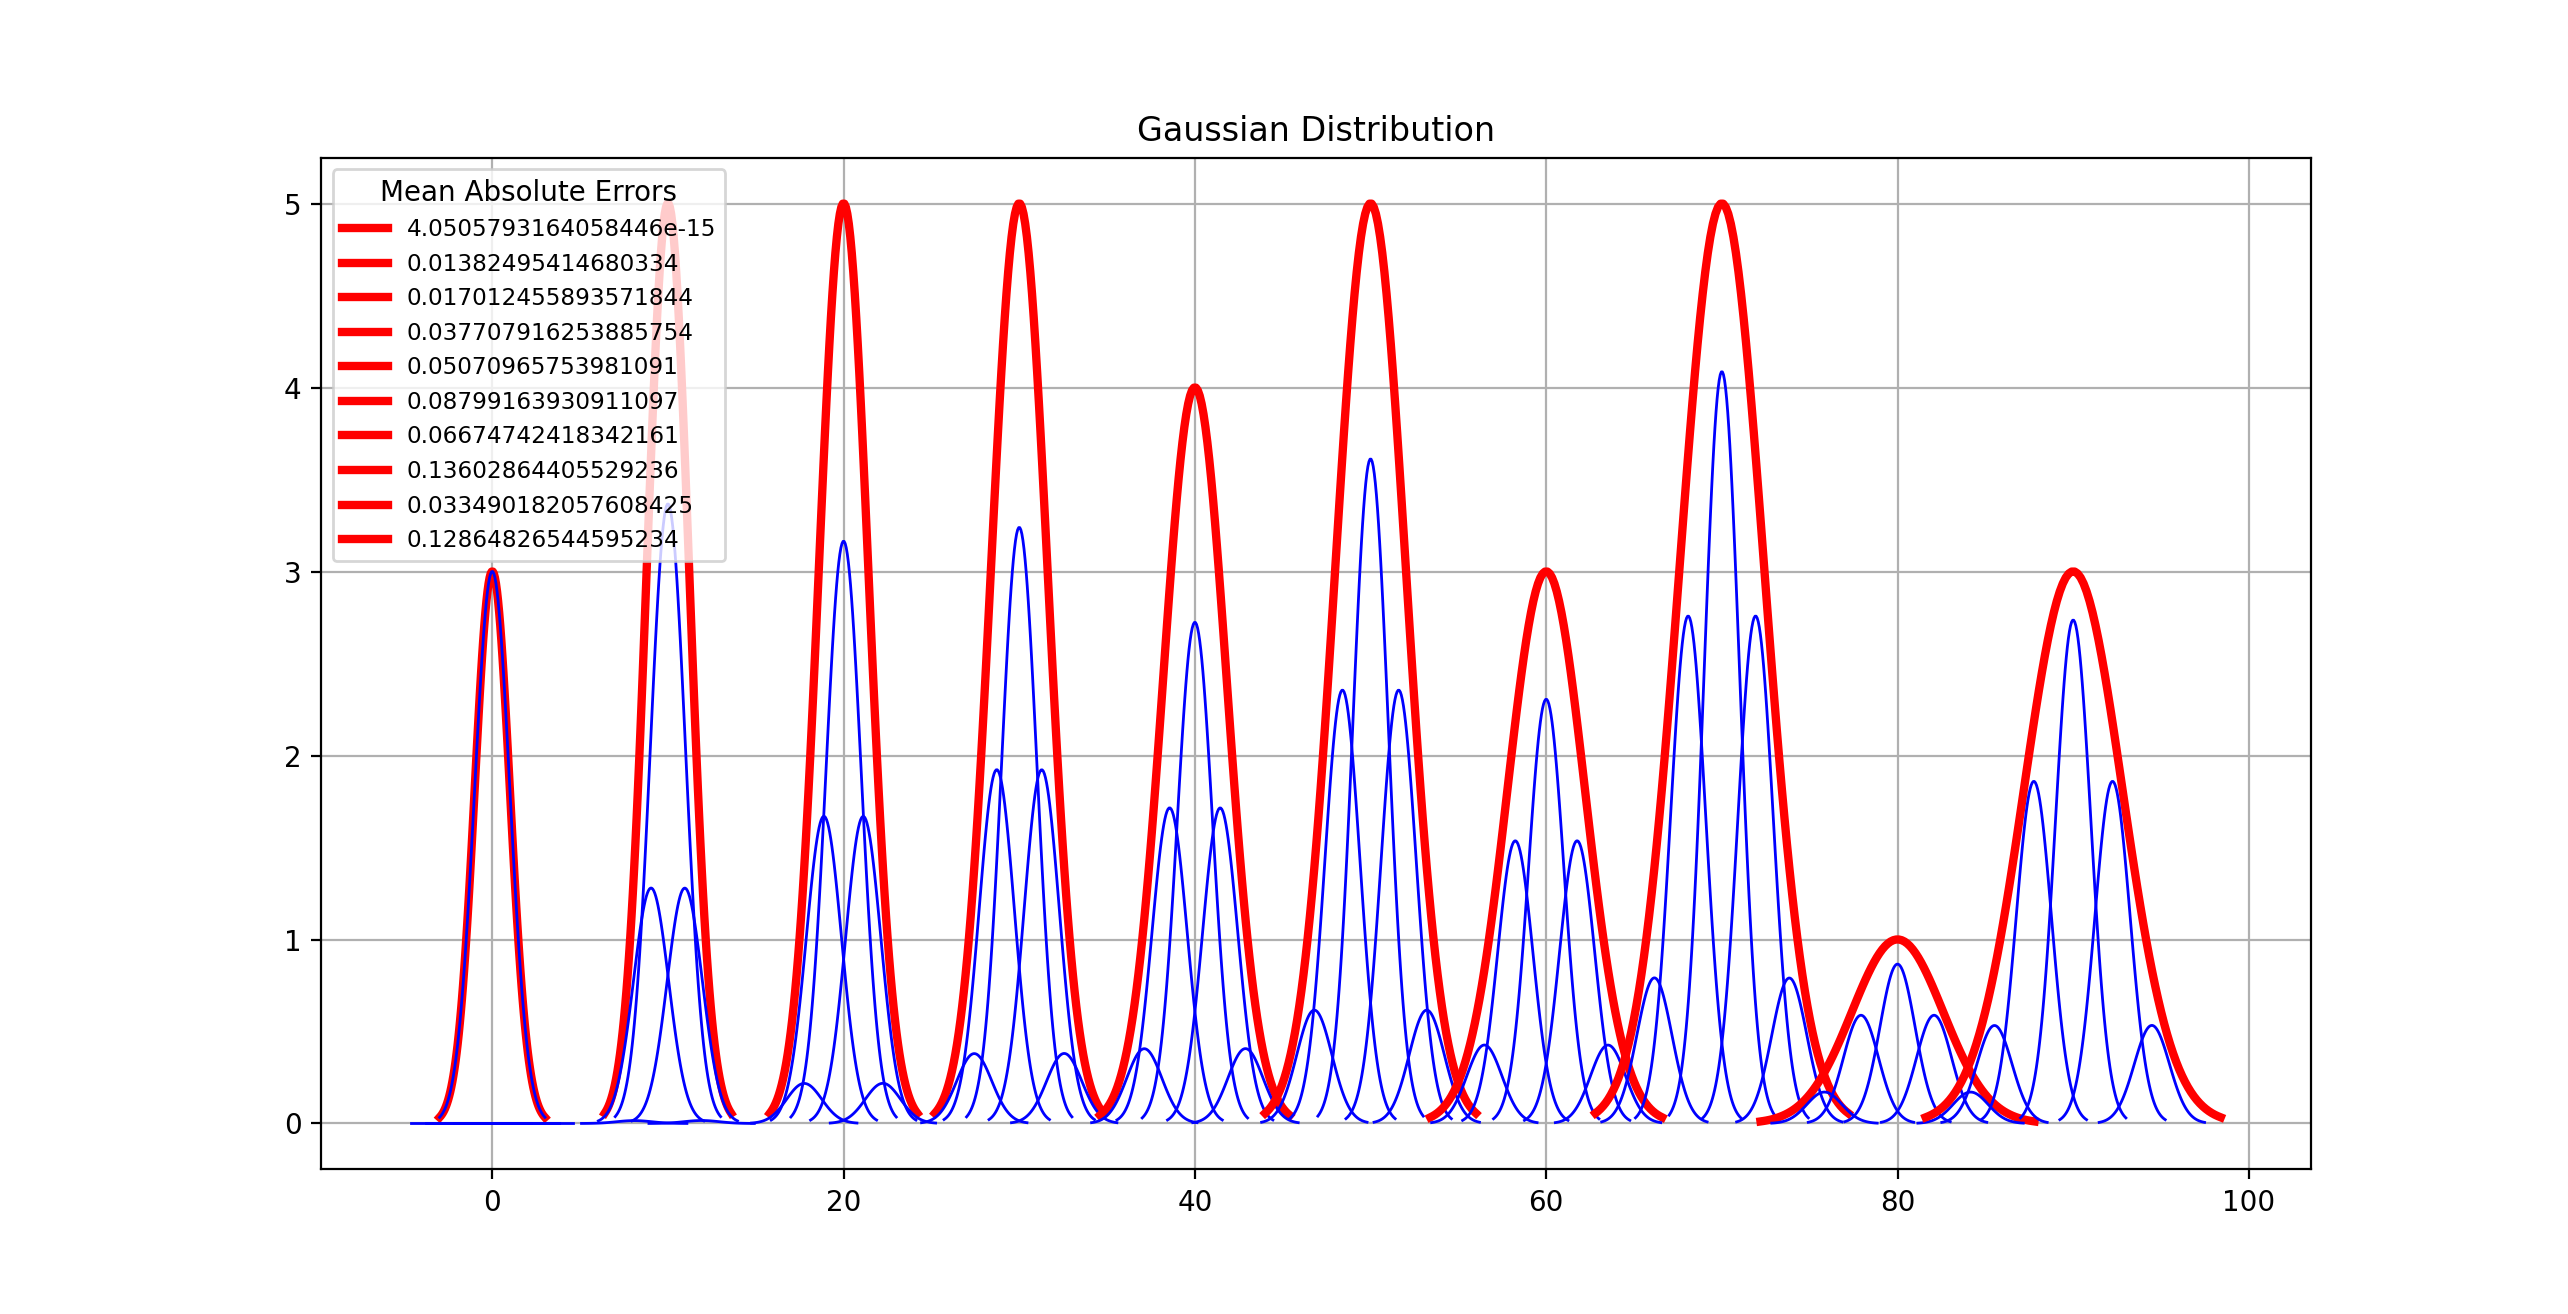
\includegraphics[scale = .6,trim= 2in 0.1in 2in 0in]{noreset.png} \\
5 mini Gaussians were generated each for 10 OGs, with the smaller standard deviation set equal to the first OG's standard deviation, and with no smaller standard deviation resets. The intensities of the OGs were generated randomly from 1-5. The standard deviations increased for the OGs from left to right from 1-3, with a step size of .2. The largest mean absolute error is about .136. However, these errors are dependent on the random generation of OGs, and vary. Here is another figure demonstrating the exact same process, with different MAEs: \\
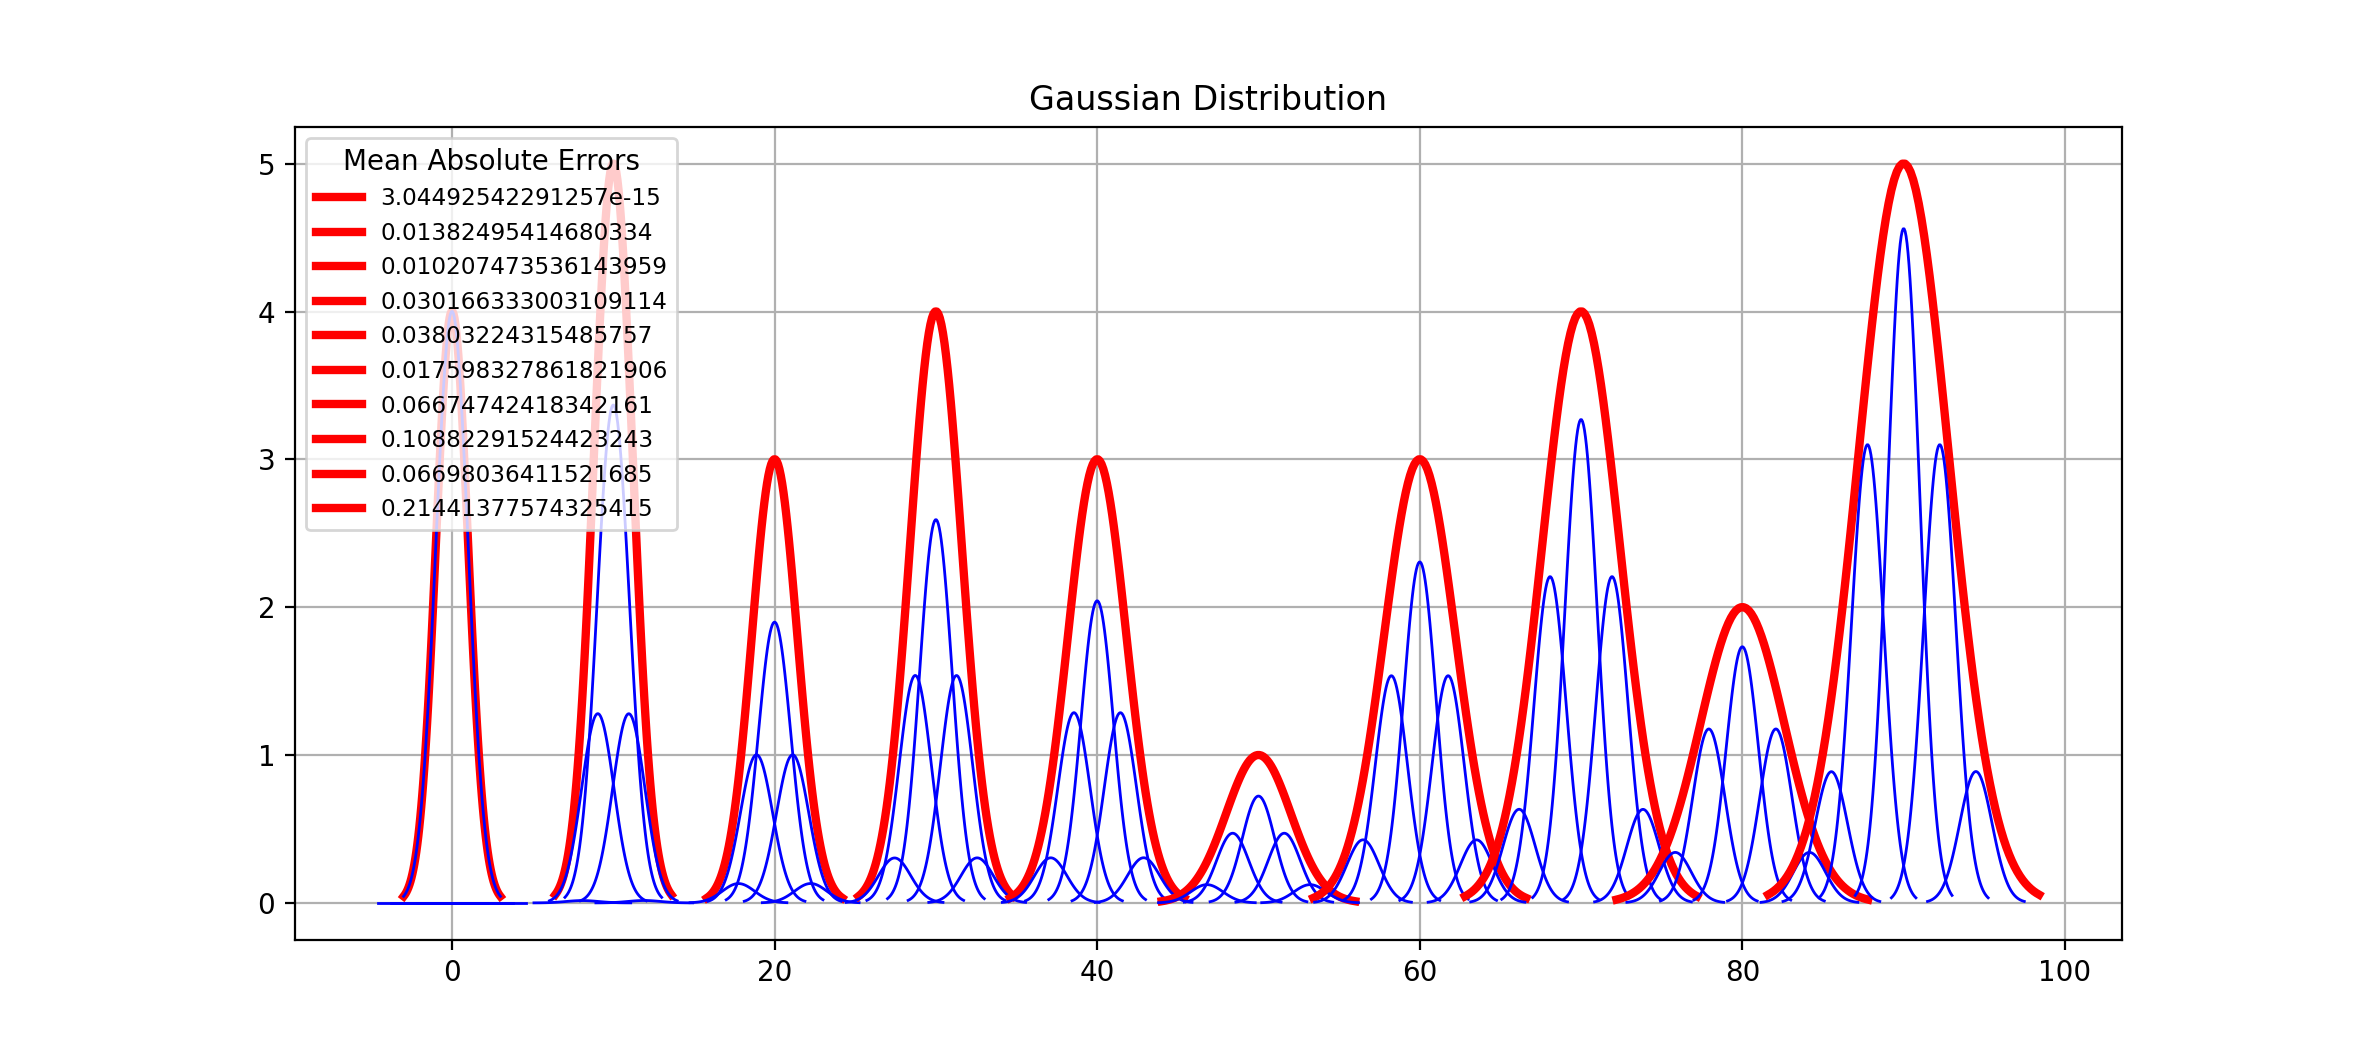
\includegraphics[scale = .6,trim= 2in 0.1in 2in 0in]{noreset2.png} \\
The last OG's approximation has a mae of .214. Below is a graph showing a seventh curve (the seventh step from the smallest standard deviation) and the final approximation (the sum of the five mini Gaussians): \\
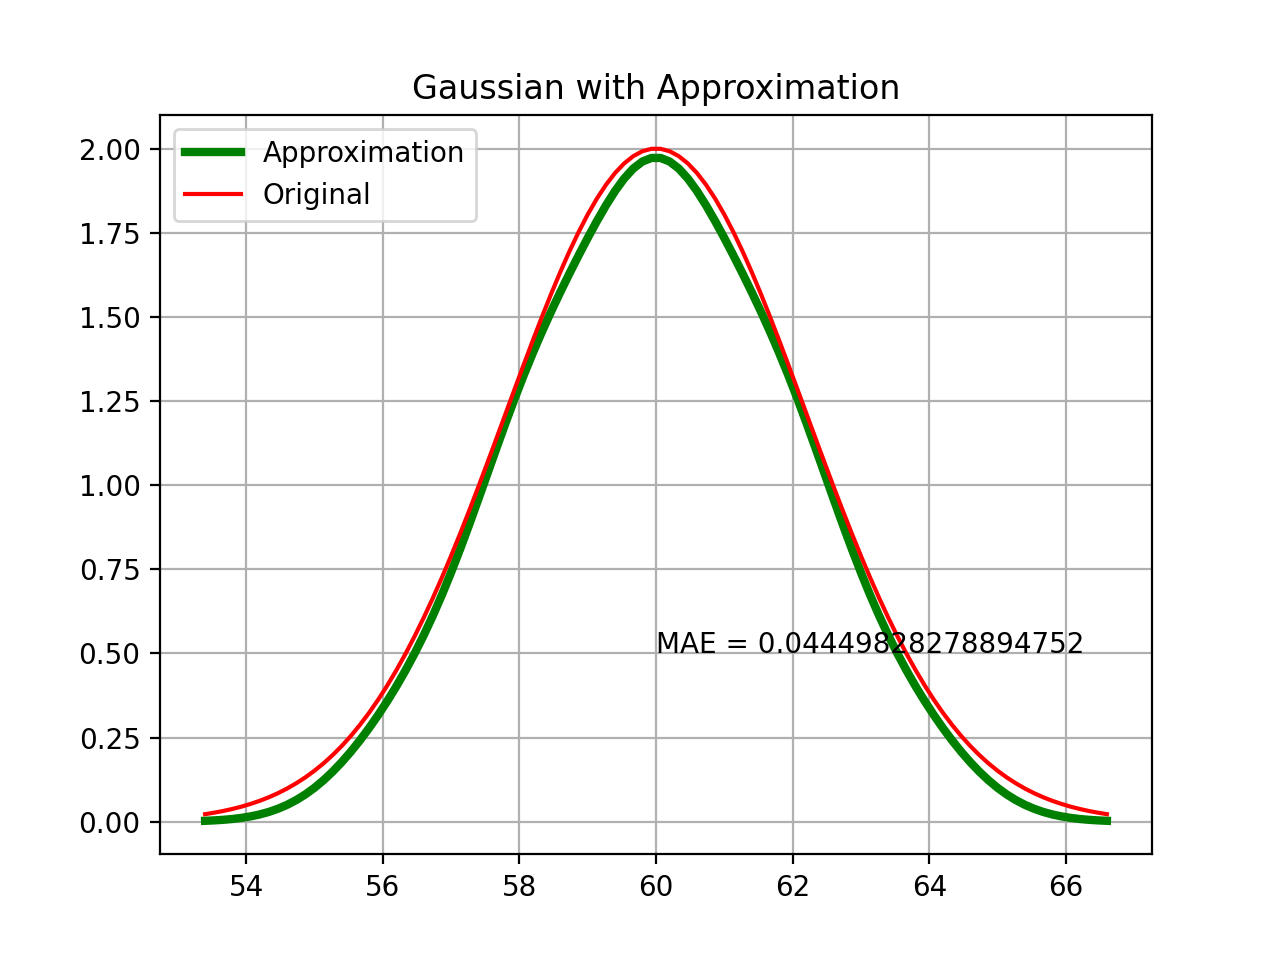
\includegraphics[scale = .8]{noreset_single.png} \\
For the constant number approach with no resets, the mean absolute error may become too high for small ratios. \\
\subsubsection*{Resets}
Next, the constant number of mini Gaussians approach with smaller standard deviation resets: \\
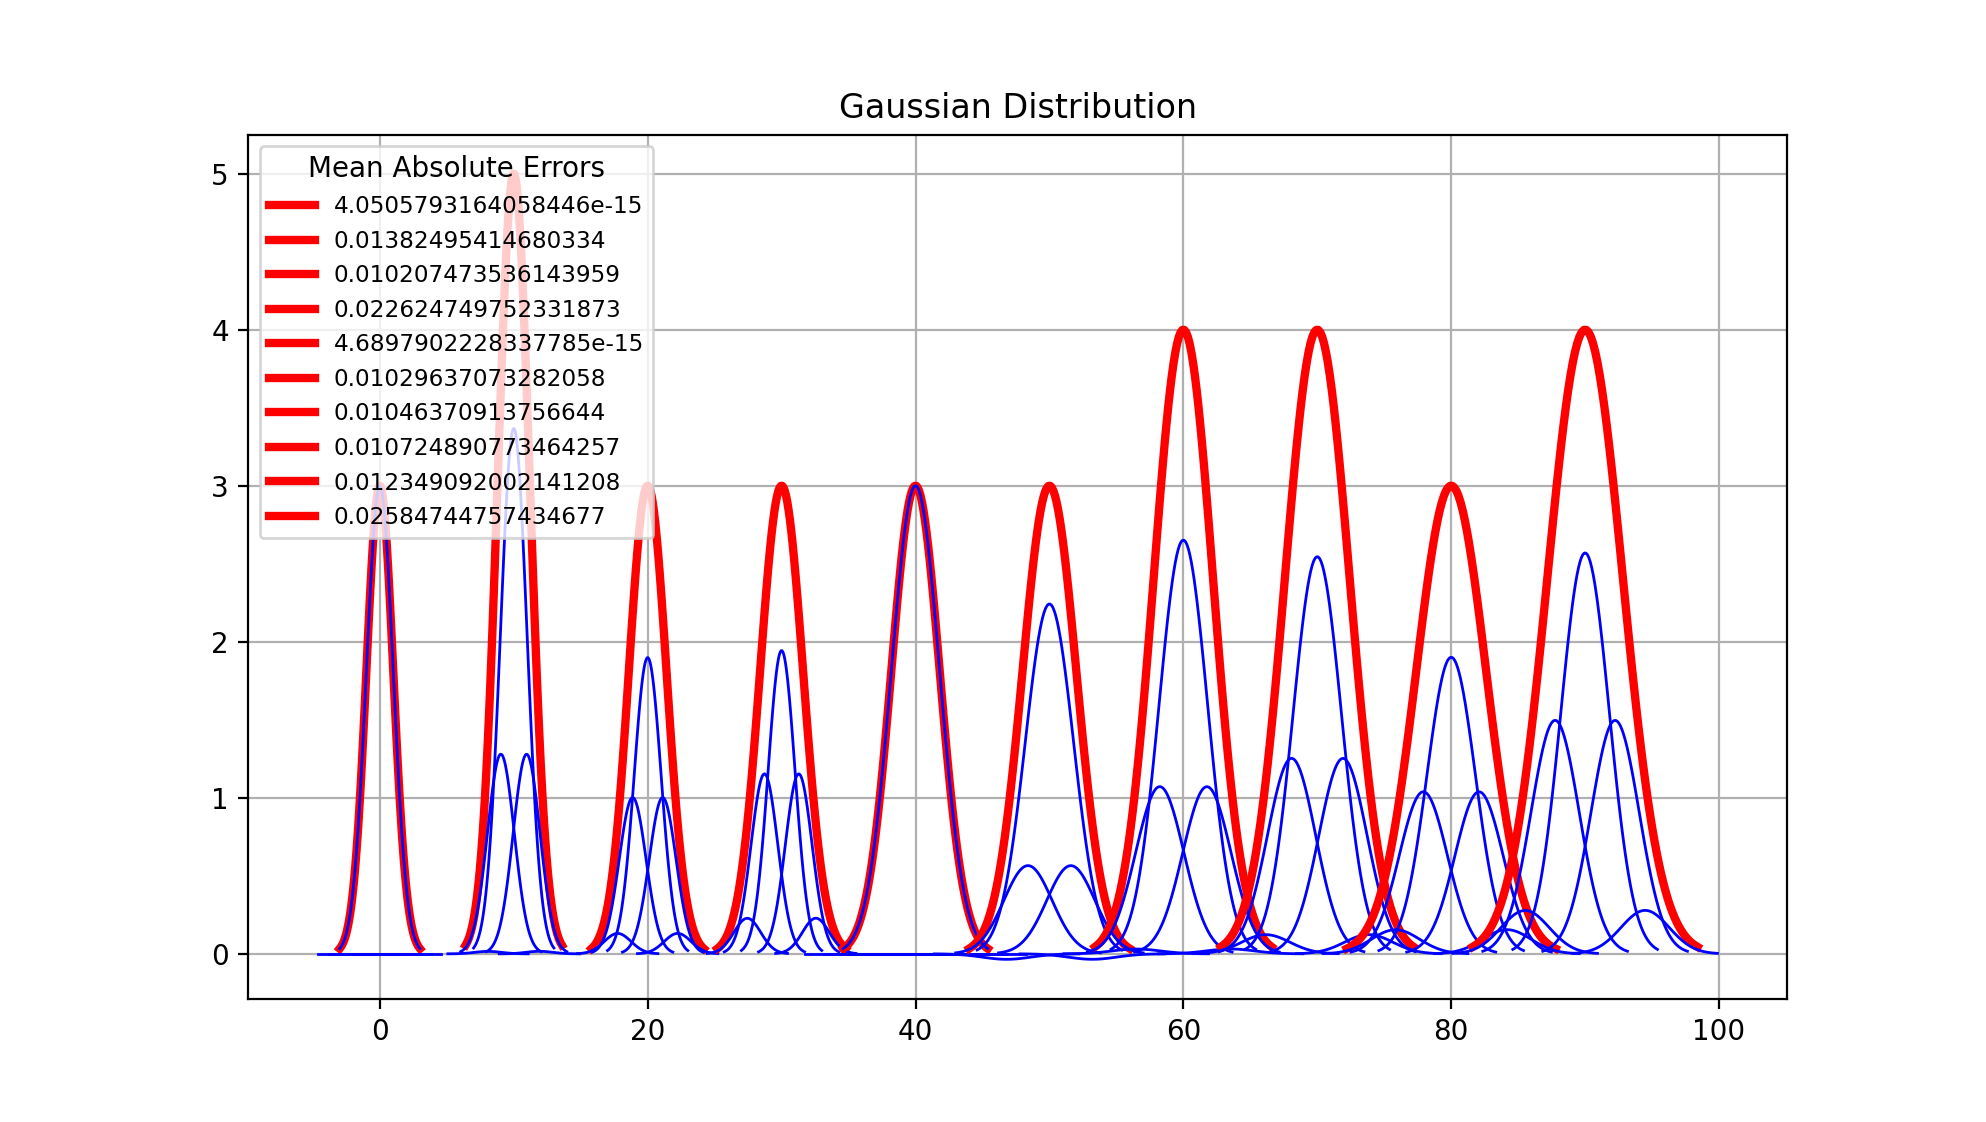
\includegraphics[scale = .8,trim= 2in 0.1in 2in 0in]{resets.png} \\
5 mini Gaussians were generated each for 10 OGs, with the smaller standard deviation set equal to the first OG's standard deviation, and with the smaller standard deviation being reset at OG number 5 (once the ratio became less than .6). The intensities of the OGs were again generated randomly from 1-5. The standard deviations increased for the OGs from left to right from 1-3, with a step size of .2. The largest mean absolute error is about .026. These errors are again dependent on the random generation of OGs, and vary. The smaller standard deviation reset occurred once the ratio was less than .6 (number taken from Coelho paper). Keeping the ratio above .6 leads to much less error in the approximations. Below is a graph showing a seventh curve (the seventh step from the smallest standard deviation) and the final approximation (the sum of the five mini Gaussians): \\
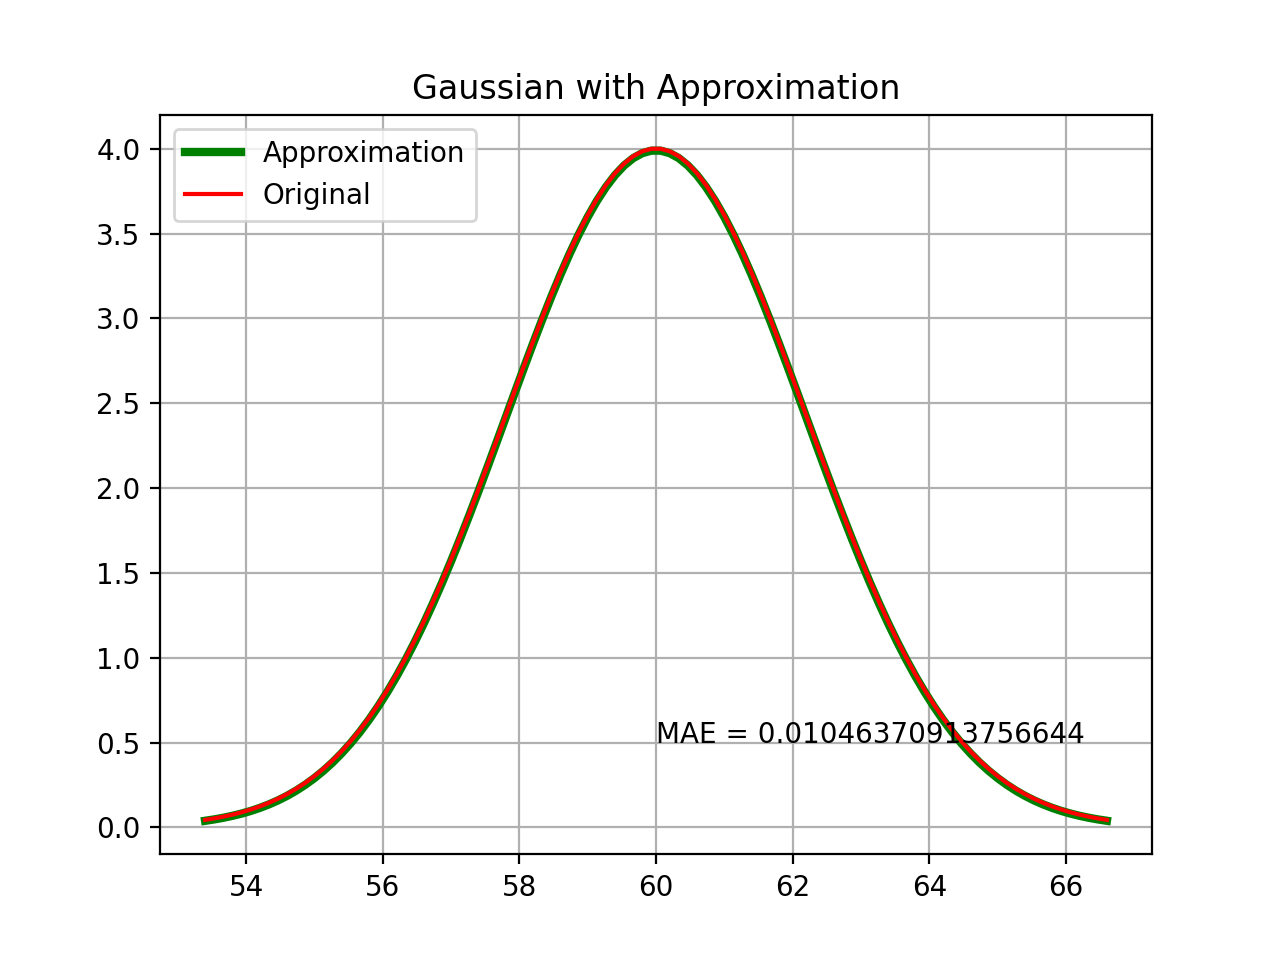
\includegraphics[scale = .8]{resets_single.png} \\
For the constant number approach with resets, the mean absolute error stays small, with the approximation almost matching the OG, as evident in the figure above. \\
\newpage
\subsection*{Method 2: Varied Number of Mini Gaussians} 
Second, the varied number of mini Gaussians approach: \\
Here are the results of two different instances of this method. \\
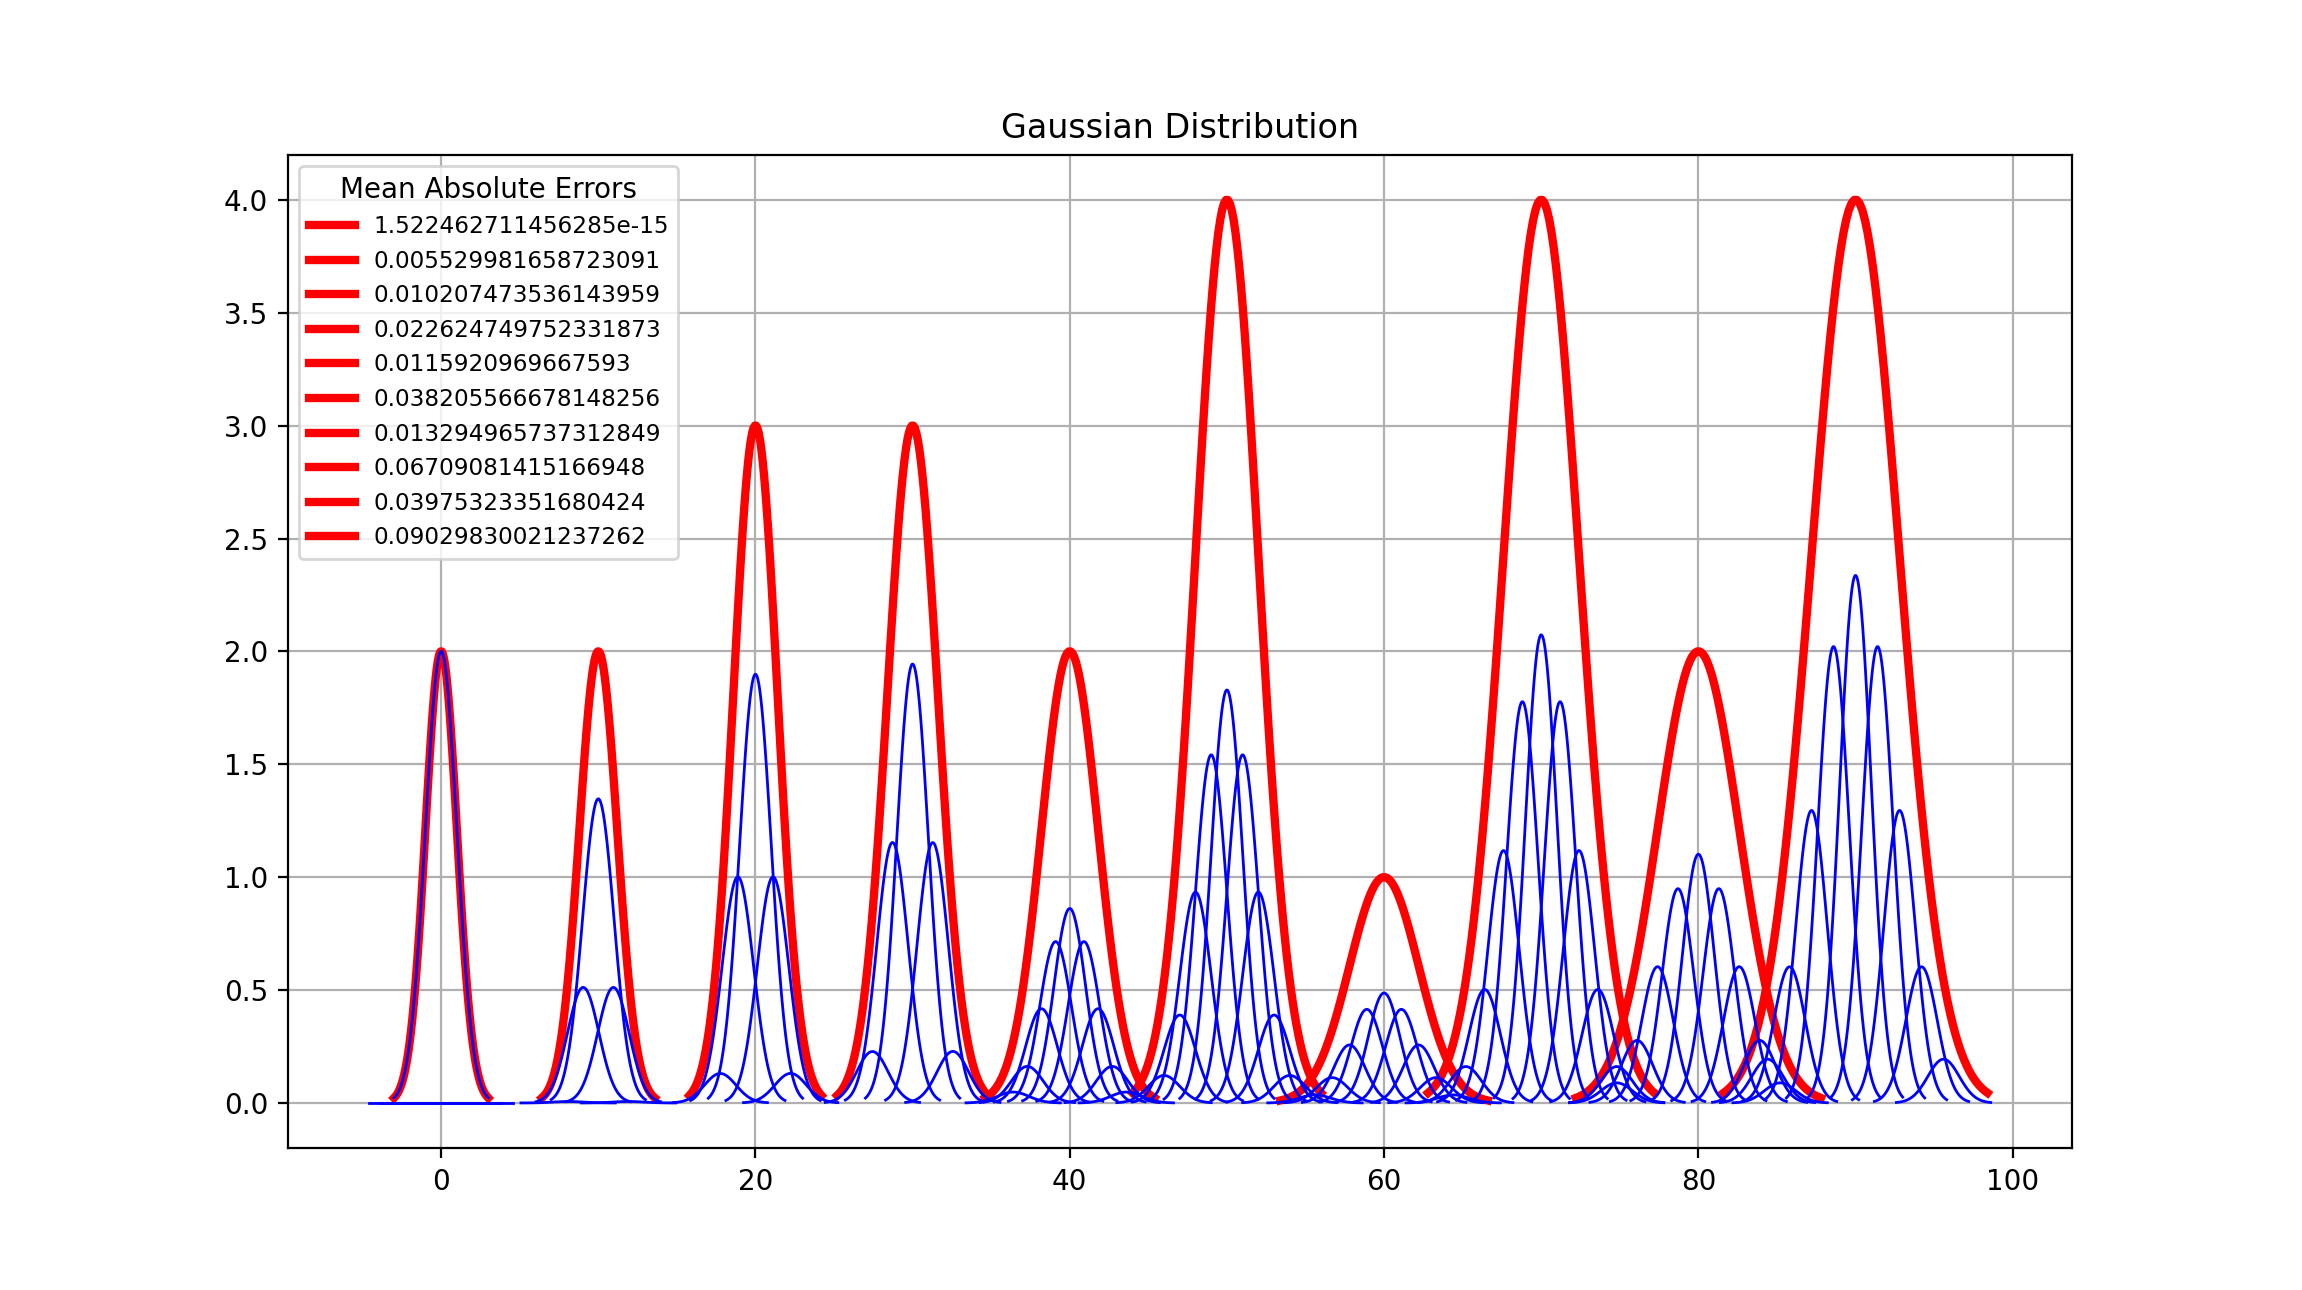
\includegraphics[scale = .6,trim= 2in 0.1in 2in 0in]{varied.png} \\
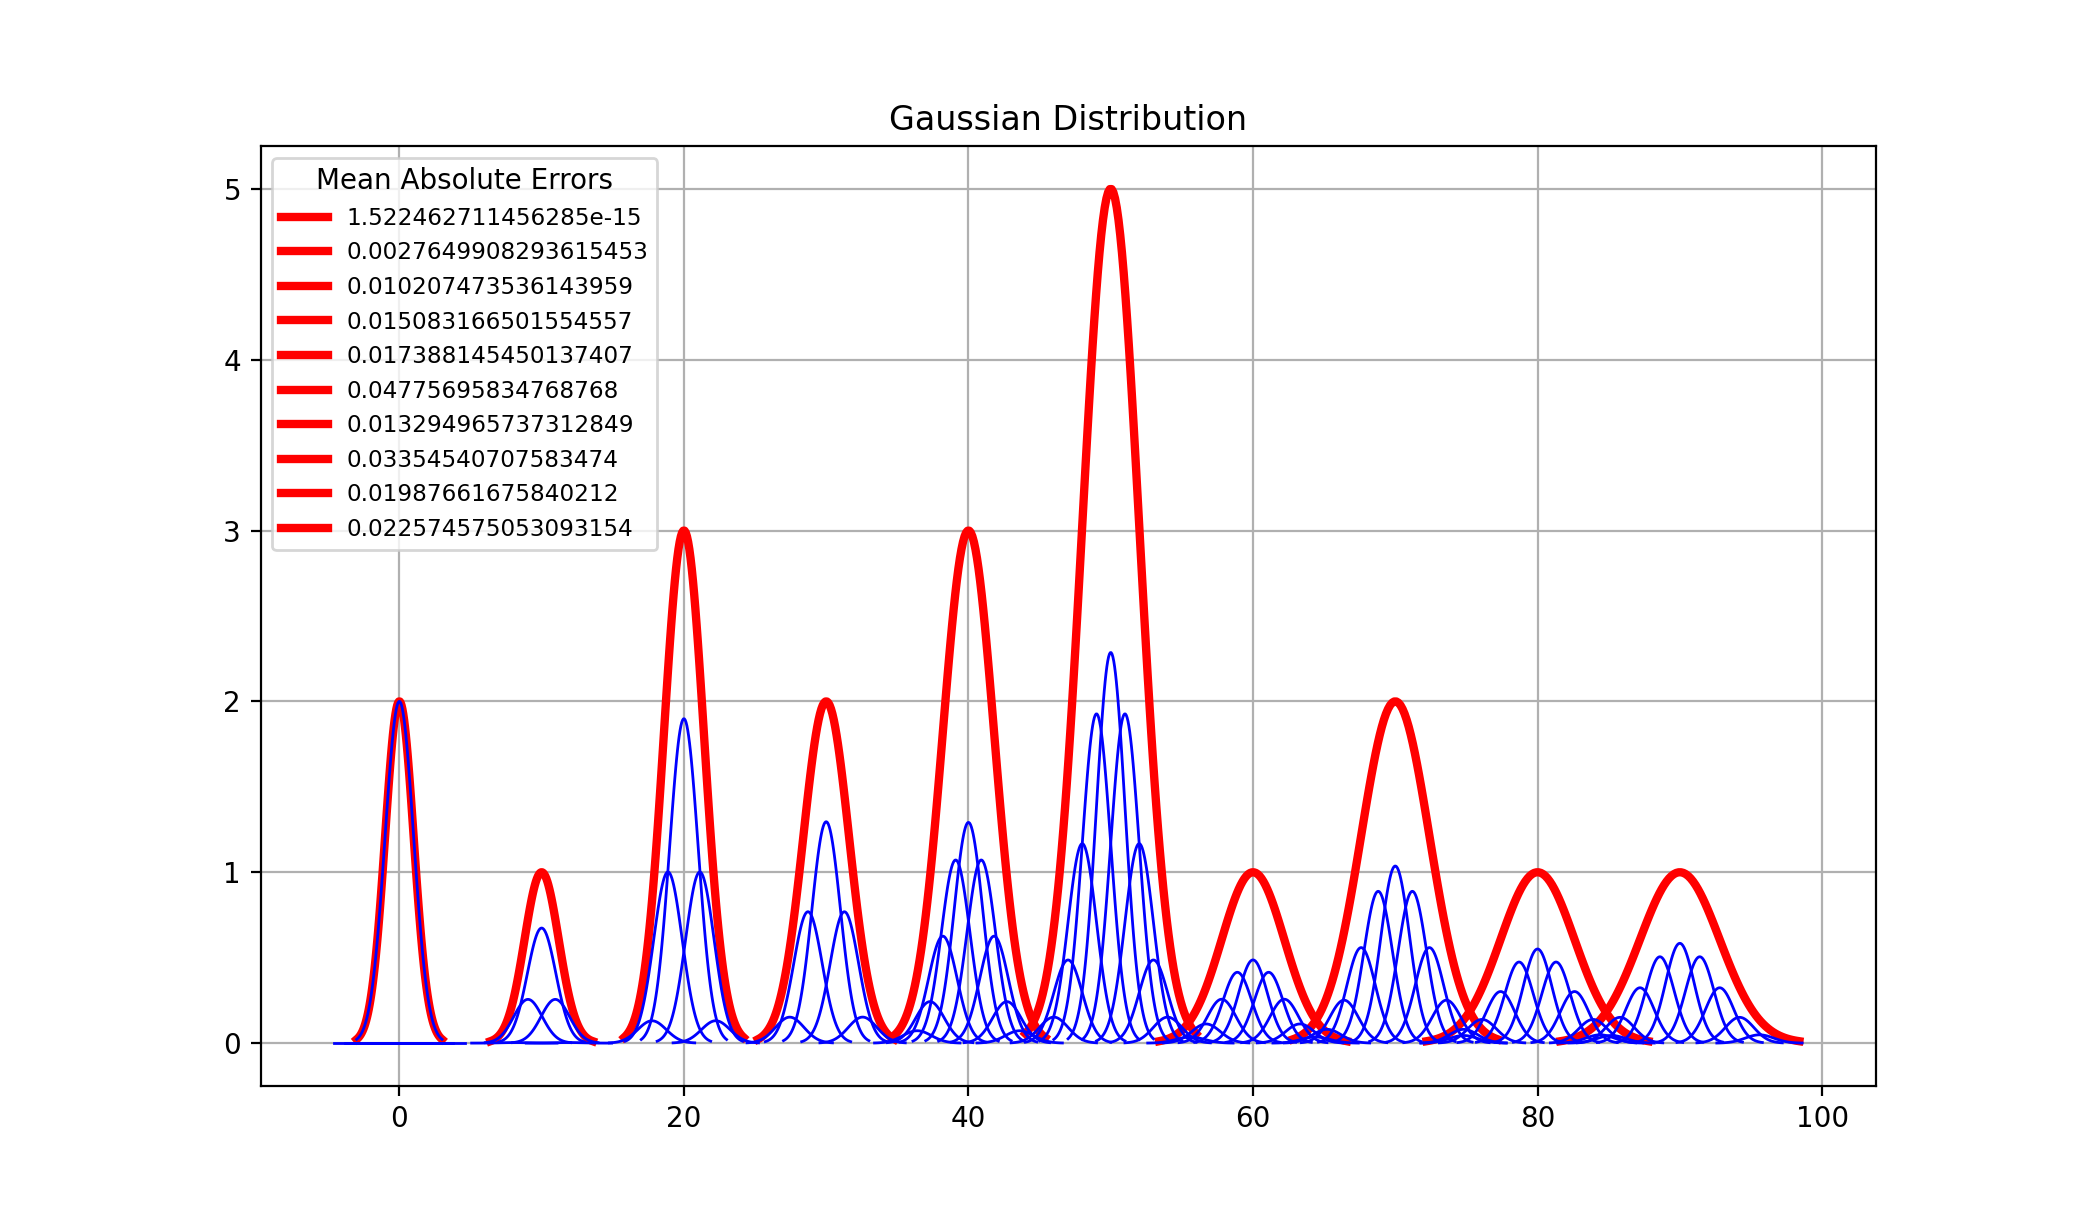
\includegraphics[scale = .6,trim= 1.5in 0.1in 2in 0in]{varied2.png} \\
The mae for this method is small. This method also requires no resets to be accurate, which is an advantage over method 1. However, one issue with this method is that right now, the only choices for the number of Gaussians is 5 or 10, based on the ratio being above or below .6. However, if the ratios in a dataset were even more drastic than the smallest ratio here (the 10th OG) of .357 (or $\frac{1}{2.8}$), then more curves may be necessary in order to generate an accurate approximation. This modification is simple, and would require a simple adjustment to the code. Below is a graph of the eighth curve (the eighth step from the smallest standard deviation) and the final approximation (the sum of the five mini Gaussians): \\
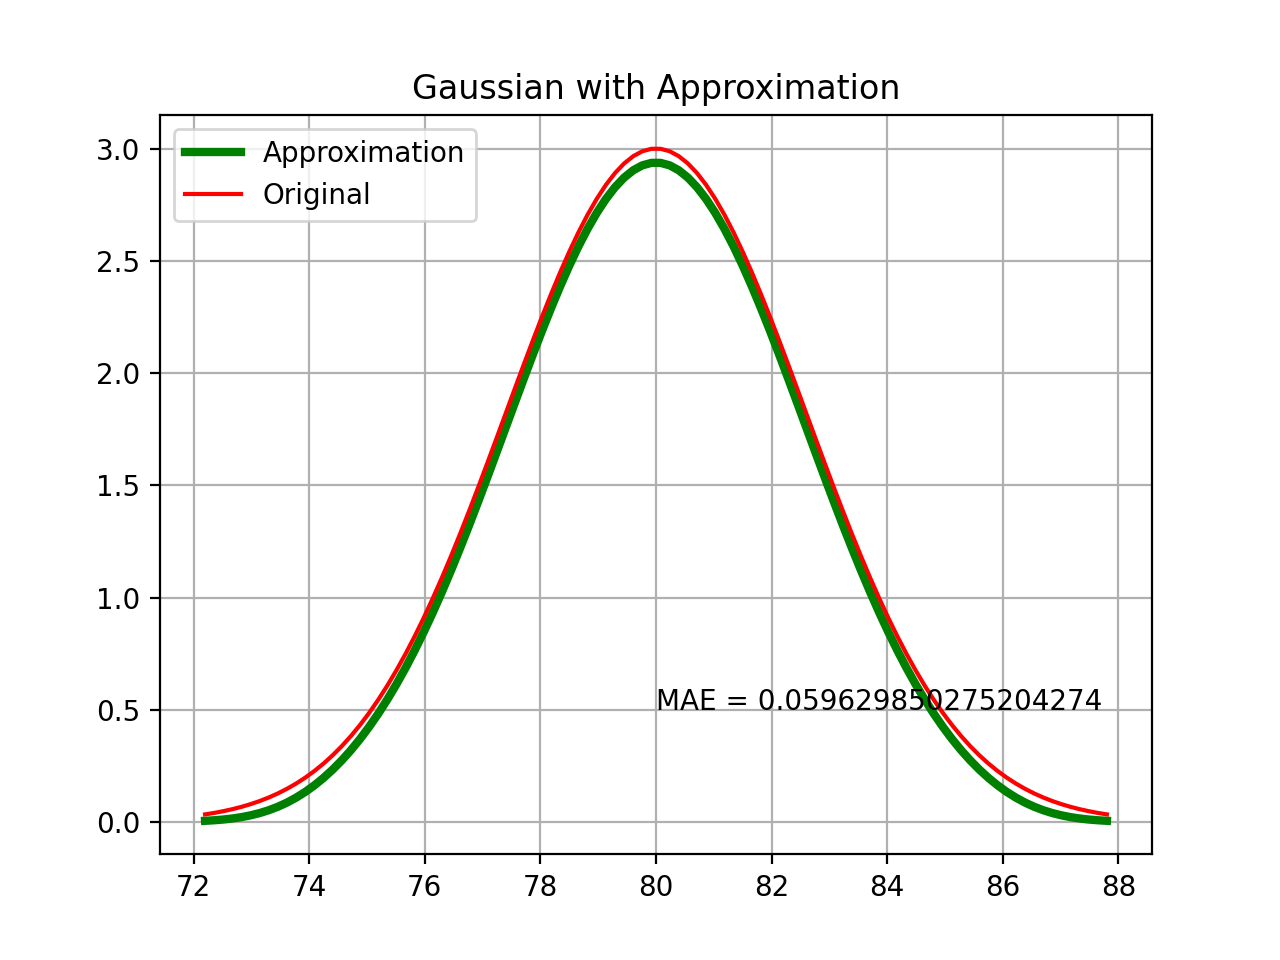
\includegraphics[scale = .8]{varied_single.png} \\
Overall, this method, since it requires no resets to guarantee accuracy, seems more promising, especially since it remains accurate for lower ratios.

\section*{Conclusions}
Both approaches, Constant Number of Mini Gaussians (without and with resets) and Varied Number of Mini Gaussians were successful in that both were able to accurately approximate Gaussian curves by generating mini Gaussians that when summed, form a close approximation to the OG. The method that should be implemented I think would ultimately depend on the dataset and the smallest ratio of the dataset. Future work would consistent of implementing the Gaussian Approximation techniques in the PDF Calculator in order to speed up the calculations.

\section*{Works Cited}
Coelho, A. A., Chater, P. A., &amp; Kern, A. (2015). Fast synthesis and refinement of the atomic pair distribution function. Journal of Applied Crystallography, 48(3), 869-875. doi:10.1107/s1600576715007487 \\

\section*{Code}
Code: \href{https://github.com/samrmayers/gaussian_work}{https://github.com/samrmayers/gaussian_work} \\
(Methods in \href{https://github.com/samrmayers/gaussian_work/blob/master/GaussApproxFINAL.py}{https://github.com/samrmayers/gaussian_work/blob/master/GaussApproxFINAL.py})


\end{document} 

